\documentclass[a4paper,11pt]{article}
\usepackage[margin=2.4cm]{geometry}
\usepackage{ctex}
\usepackage{amsmath,amssymb}
\usepackage{booktabs}
\usepackage{multirow}
\usepackage{array}
\usepackage{makecell}
\usepackage{siunitx}
\usepackage{xcolor}
\usepackage{hyperref}
\usepackage{enumitem}
\usepackage{float}
\usepackage{graphicx}

\hypersetup{colorlinks=true, linkcolor=blue!60!black, citecolor=blue!60!black, urlcolor=blue!60!black}

\title{\textbf{NN proton 重建: ypol + zpol breakup g4output 的 R / $\Delta p_x$ 物理观测}}
\author{Baiting Tian \\ RIKEN 仁科中心 / DPOL 实验}
\date{2026 年 5 月 3 日}

\begin{document}
\maketitle

\section*{摘要}
本报告把 PDC$\to$target proton 主 NN 模型 (\texttt{formal\_B115T3deg/20260420\_184345}) 应用到 spana03 上 ypol 和 zpol 的 breakup g4output (Sn112E190/Sn124E190 $\times$ g050/g060/g070/g080 $\times$ ynp/ypn 或 znp/zpn, 共 32 cell, ypol 4.59M 事件 / zpol 0.10M 事件), 重建 proton 动量, 并把 NEBULA 重建的 neutron 拼起来,
按照 \texttt{ypol\_phys\_20260428\_zh.tex} 同口径在三种 input\_ana cut (loose/mid/tight) 下统计反应平面 frame 的 $\Delta p_x^\text{rot}$ 分布与 $R = N(\Delta p_x^\text{rot}>0)/N(\Delta p_x^\text{rot}<0)$.
\textbf{关键结果}: 在 ypol Sn124 上 R 随 gamma 单调下降 (loose 0.29$\to$0.23; tight 0.57$\to$0.32), Sn112 趋势更弱; zpol Sn124 上 R 也表现出强 gamma 依赖 (loose 0.95$\to$0.31), Sn112 数据有限. NN 重建 (mixed) 与 truth 在所有 cell × cut 上一致到 $<5\%$, 验证 NN proton + truth-fallback neutron 是可用的物理观测路径.
\textbf{后续报告独立分两份}: (i) 同样数据上 RK 重建结果（在 spana03 上跑后另出一份）, (ii) NN vs RK 头对头比较报告.

\section{1. 主模型}

模型 ID: \texttt{data/nn\_target\_momentum/formal\_B115T3deg/20260420\_184345}.
完整训练细节、自检指标、结构 (6$\to$128/128/64$\to$3 MLP, 隐藏 ReLU) 见 \texttt{nn\_vs\_rk\_ypol\_allair\_20260503\_zh.tex} §1.
本报告只需关心一个边界条件: 训练域是 $(p_x, p_y)$ 半径 $R \le 100$ MeV/$c$ 圆盘 + $p_z \in [560, 680]$ MeV/$c$. breakup 事件相对 elastic 有更宽的 $p_T$ 与 $p_z$ 分布, 训练域覆盖率见 §4.

\section{2. 数据流}

\subsection*{2.1 数据来源}
spana03 路径:
\begin{verbatim}
/home/tbt/workspace/Dpol_smsimulator/data/simulation/g4output/y_pol/phi_random/<cell>/dbreak0000.root
/home/tbt/workspace/Dpol_smsimulator/data/simulation/g4output/z_pol/b_discrete/<cell>/dbreakb{01..10}0000.root
\end{verbatim}
通过 \texttt{rsync} 1:1 镜像到本地 \texttt{data/simulation/g4output/\{y\_pol,z\_pol\}/} (脚本本地远程通用):
\begin{itemize}[nosep]
    \item ypol: 16 cell, 每 cell 一个 \texttt{dbreak0000.root}, 总计 7.2 GB
    \item zpol: 16 cell × 10 b-段, 每 cell 总计 8.5--43 MB, 总计 269 MB
\end{itemize}

\subsection*{2.2 NN 重建}
对每个 sampled root 跑一次:
\begin{verbatim}
build/bin/reconstruct_target_momentum \
  --input-file <g4output> \
  --output-file data/reconstruction/breakup_nn_20260503/<pol>/<cell>[_bNN]_reco_nn.root \
  --geometry-macro configs/.../geometry_B115T_pdcOptimized_20260227_target3deg.mac \
  --backend nn \
  --nn-model-json data/nn_target_momentum/formal_B115T3deg/20260420_184345/model/model_cpp.json
\end{verbatim}
geometry macro 与训练时一致, 靶倾角 $3°$. 6 路并行, 全 32 cell × 176 reco 任务总耗时 97 s.

\subsection*{2.3 Neutron 来源}
NN backend 只重建 proton, neutron 仍走原 \texttt{NEBULAReconstructor} ($\beta$ 法 + commit \texttt{806cd6a} 的 \texttt{NEBULAFrameRotation::RotateRecoNeutronsToTargetFrame}, 详见 \texttt{ypol\_phys\_20260428\_zh.tex} §2.3).

\subsection*{2.4 抽取 \& 拼接}
\texttt{02\_extract\_observables.C} 把每 reco root 的 truth + NN proton + NEBULA neutron 写到一行 CSV,
zpol 的 10 个 b-段被 append 到同一份 cell CSV (保留 \texttt{b\_segment} 列). 每 cell 一份 CSV, 共 32 份.

\subsection*{2.5 反应平面定义}
对每事件用 \textbf{truth} 总横向动量定义反应平面:
\[
    \phi^\text{event} = \arctan_2(\,p_{y,p}^\text{truth} + p_{y,n}^\text{truth},\;\; p_{x,p}^\text{truth} + p_{x,n}^\text{truth}\,)
\]
然后对 $(p_x, p_y)$ 旋转 $-\phi$, 让 $\vec p_T^\text{sum}$ 对齐到 $+\hat x$ 方向. 所有后续 $\Delta p_x^\text{rot}$ 都在反应平面 frame 下.

\subsection*{2.6 三档 reco-variant (与 elastic 报告一致)}
\begin{tabular}{lp{12cm}}
\toprule
\textbf{A. truth}       & \texttt{truth\_pxp} - \texttt{truth\_pxn} (truth 旋转后差) \\
\textbf{B. reco mixed}  & NN proton 旋转后 $p_x$ 减 \{NEBULA-hit 时 reco neutron, 否则 truth neutron\} 旋转后 $p_x$ \\
\textbf{C. full reco}   & NN proton − reco neutron, 仅在 NEBULA-hit 子集上 \\
\bottomrule
\end{tabular}

\subsection*{2.7 通过率}
\begin{table}[H]
\centering\footnotesize
\begin{tabular}{lr}
\toprule
项目 & 计数 \\
\midrule
ypol total g4output 事件        & 4\,588\,274 \\
\quad NN proton OK (status==0)  & 3\,382\,925 (73.7\%) \\
zpol total g4output 事件        & 161\,839 \\
\quad NN proton OK              & 101\,662 (62.8\%) \\
\bottomrule
\end{tabular}
\end{table}
\textbf{读法}: PDC 击中决定 NN proton 是否输出. 73\% (ypol) / 63\% (zpol) 的事件具备完整 PDC1+PDC2 击中, NN forward 100\% 给出有效输出.

\section{3. Cut 定义}

引用 \texttt{scripts/notebooks/input\_analysis/core/cuts.py}, 在 truth 量上施加:

\paragraph{ypol cuts}
\begin{itemize}[nosep]
    \item \textbf{loose}: $|p_{y,p} - p_{y,n}| < 150$ \textbf{且} $|\vec p_T^\text{sum}|^2 > 2500$
    \item \textbf{mid}:   loose \textbf{且} $(\text{rot\_pxp} + \text{rot\_pxn}) < 200$
    \item \textbf{tight}: mid \textbf{且} $(\pi - |\phi^\text{event}|) < 0.2$
\end{itemize}

\paragraph{zpol cuts}
\begin{itemize}[nosep]
    \item \textbf{loose}: $(p_{z,p} + p_{z,n}) > 1150$ \textbf{且} $|p_{z,p} - p_{z,n}| < 150$
    \item \textbf{mid}:   loose \textbf{且} $(p_{x,p} + p_{x,n}) < 200$ \textbf{且} $|\vec p_T^\text{sum}|^2 > 2500$
    \item \textbf{tight}: mid \textbf{且} $(\pi - |\phi^\text{event}|) < 0.5$
\end{itemize}

注意 zpol 的 loose 主要靠 $p_z$ 重质心, 通过率几乎 100\% (见 §5.1); ypol loose 才是真正在筛 in-plane 事件.

\section{4. 训练域 vs breakup truth}

\begin{table}[H]
\centering\footnotesize
\caption{breakup truth 中落入 NN 训练域的事件比例.}
\begin{tabular}{lcc}
\toprule
                         & ypol & zpol \\
\midrule
$p_T \le 100$ MeV/$c$    & 97.5\% & 91.5\% \\
$p_z \in [560, 680]$     & 99.6\% & 99.5\% \\
两者同时                  & \textbf{97.4\%} & \textbf{91.3\%} \\
\bottomrule
\end{tabular}
\end{table}

\textbf{结论}: ypol 几乎全在训练域内, NN 推理可信; zpol 有 $\sim$9\% 事件在 $p_T > 100$ 的外推区. 后续 NN-vs-RK 比较报告中可重点考察这部分外推事件.

\section{5. ypol 章节}

\subsection{5.1 通过率 (ynp+ypn 已合并)}

\begin{table}[H]
\centering\footnotesize
\caption{ypol per-(target, gamma) 通过率 (基于 truth cuts, 两 helicity pool). N\_NEBULA(in tight) = tight 子集中 NEBULA 击中数.}
\begin{tabular}{llrrrrr}
\toprule
target & gamma & N\_raw & N\_loose & N\_mid & N\_tight & N\_NEBULA(in tight) \\
\midrule
Sn112E190 & g050 & 239\,349 & 123\,311 & 105\,189 &  9\,999 & 1\,852 \\
Sn112E190 & g060 & 385\,635 & 120\,036 & 101\,134 & 11\,703 & 2\,257 \\
Sn112E190 & g070 & 475\,908 & 118\,057 &  98\,923 & 12\,562 & 2\,283 \\
Sn112E190 & g080 & 600\,569 & 117\,829 &  98\,215 & 13\,522 & 2\,544 \\
Sn124E190 & g050 & 214\,559 & 120\,733 & 103\,071 &  8\,950 & 2\,213 \\
Sn124E190 & g060 & 359\,926 & 116\,800 &  99\,006 & 10\,368 & 2\,462 \\
Sn124E190 & g070 & 512\,280 & 116\,737 &  98\,462 & 11\,710 & 2\,651 \\
Sn124E190 & g080 & 594\,699 & 117\,227 &  98\,476 & 12\,513 & 2\,782 \\
\bottomrule
\end{tabular}
\end{table}

\textbf{读法}: tight 通过率 $\sim 2$--$5\%$; NEBULA 在 tight 子集上击中率 $\sim 18$--$22\%$.

\subsection{5.2 R 表 (ypol, $R_x^\text{rot}$ per (target, gamma) × cut × variant)}

R 单元格格式: $R$\,[$R_{16}, R_{84}$] (1000 次 bootstrap 68\% CI).

\begin{table}[H]
\centering\scriptsize
\caption{ypol $R_x^\text{rot}$ (反应平面 frame, ynp+ypn pooled).}
\begin{tabular}{ll|ccc|ccc|ccc}
\toprule
& & \multicolumn{3}{c|}{\textbf{loose}} & \multicolumn{3}{c|}{\textbf{mid}} & \multicolumn{3}{c}{\textbf{tight}} \\
target & gamma & A truth & B mixed & C full & A truth & B mixed & C full & A truth & B mixed & C full \\
\midrule
Sn112 & g050 & 0.226 & 0.225 & 0.755 & 0.249 & 0.253 & 0.740 & 0.308 & 0.313 & 1.156 \\
Sn112 & g060 & 0.226 & 0.226 & 0.768 & 0.252 & 0.256 & 0.755 & 0.263 & 0.267 & 0.919 \\
Sn112 & g070 & 0.217 & 0.216 & 0.737 & 0.242 & 0.246 & 0.729 & 0.226 & 0.229 & 0.758 \\
Sn112 & g080 & 0.212 & 0.212 & 0.705 & 0.238 & 0.242 & 0.696 & 0.219 & 0.221 & 0.719 \\
Sn124 & g050 & 0.291 & 0.292 & 0.979 & 0.329 & 0.335 & 0.975 & 0.566 & 0.571 & 1.830 \\
Sn124 & g060 & 0.265 & 0.266 & 0.915 & 0.300 & 0.305 & 0.911 & 0.475 & 0.481 & 1.462 \\
Sn124 & g070 & 0.245 & 0.245 & 0.821 & 0.276 & 0.281 & 0.821 & 0.377 & 0.381 & 1.079 \\
Sn124 & g080 & 0.228 & 0.229 & 0.792 & 0.256 & 0.260 & 0.783 & 0.316 & 0.320 & 0.891 \\
\bottomrule
\end{tabular}
\end{table}

完整 bootstrap CI 见 \texttt{build/test\_output/nn\_breakup\_phys\_20260503/summary/ypol/r\_table.csv}; 所有 CI 宽度 $<3\%$ 相对值 (统计精度足够).

\textbf{物理结论}:
\begin{itemize}[nosep]
    \item \textbf{Sn124 的 R 随 gamma 单调下降}, tight cut 下从 0.57 (g050) 跌到 0.32 (g080) — 信号清晰.
    \item \textbf{Sn112 趋势弱}, loose/mid 几乎不随 gamma 变, tight 在 g060 附近转折但幅度小.
    \item \textbf{B mixed 与 A truth 一致到 $<3\%$} 的相对偏差, 证明 NN proton 重建在反应平面 R 这个观测量上没有显著系统偏 (尽管 NN 的 px 中位数有 $-0.8$ MeV/c 的偏, 见 §5.4).
    \item \textbf{C full reco 因 NEBULA 接收度偏置整体偏高}, lab-frame 与 reaction-plane frame 不直接可比 (与 elastic 报告 §7 同一原因).
\end{itemize}

\subsection{5.3 ypol R 与 $\Delta p_x^\text{rot}$ 图}

\begin{figure}[H]
\centering
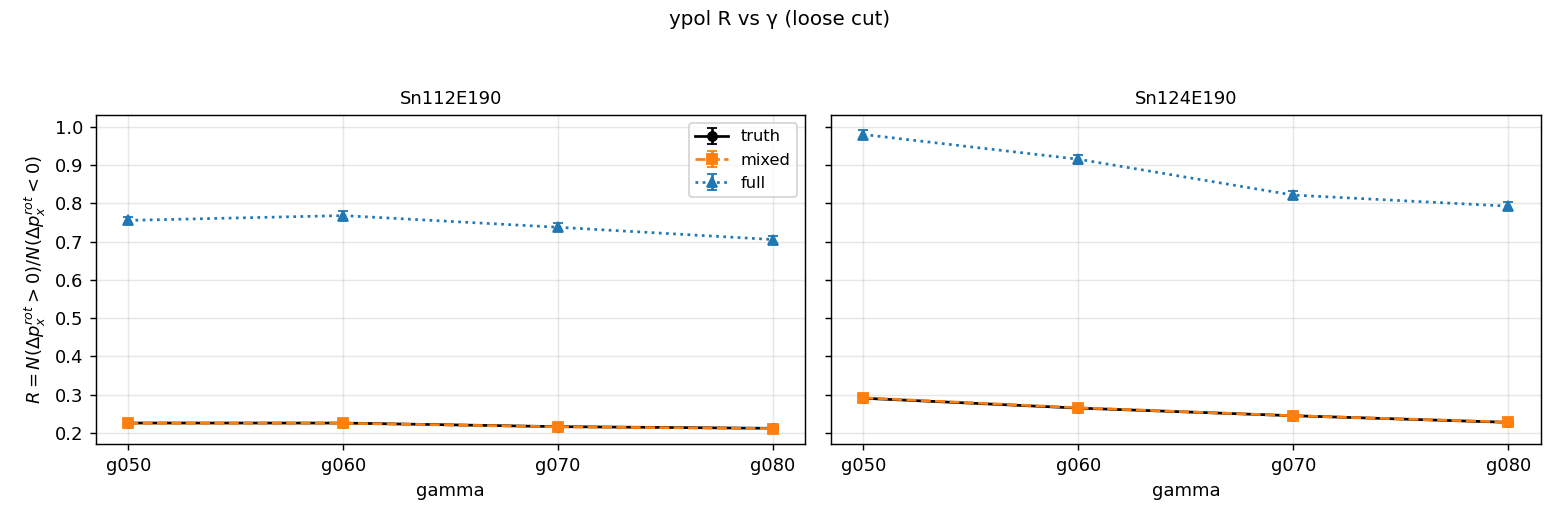
\includegraphics[width=0.95\textwidth]{figures/nn_breakup_phys/r_vs_gamma_ypol_loose.png}
\caption{ypol $R_x^\text{rot}$ vs gamma (loose cut). 黑圆 = A truth, 橙方虚 = B NN mixed, 蓝三角点 = C NN full. error bar = 68\% bootstrap CI.}
\end{figure}
\begin{figure}[H]
\centering
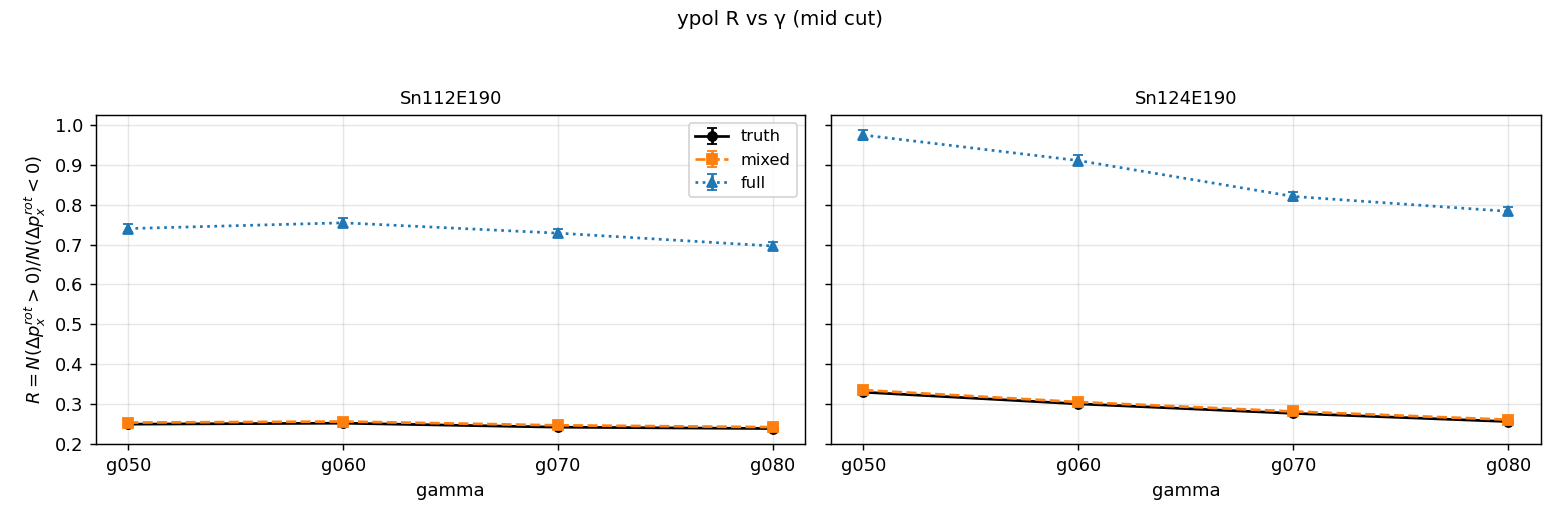
\includegraphics[width=0.95\textwidth]{figures/nn_breakup_phys/r_vs_gamma_ypol_mid.png}
\caption{ypol $R_x^\text{rot}$ vs gamma (mid cut).}
\end{figure}
\begin{figure}[H]
\centering
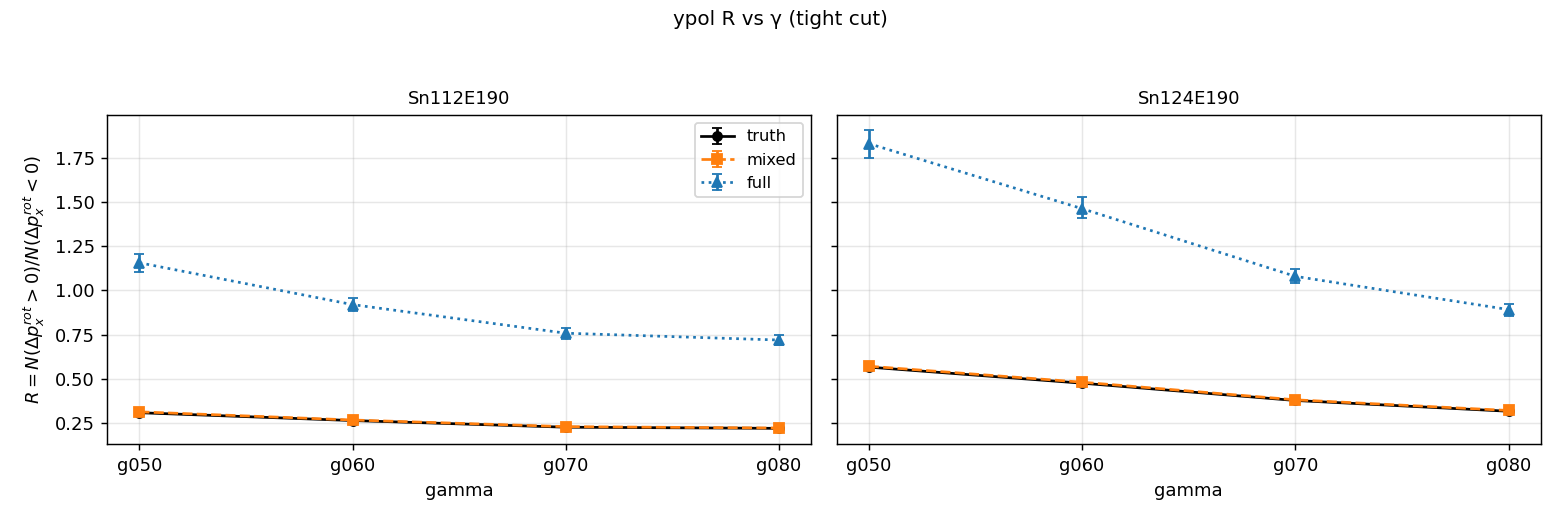
\includegraphics[width=0.95\textwidth]{figures/nn_breakup_phys/r_vs_gamma_ypol_tight.png}
\caption{ypol $R_x^\text{rot}$ vs gamma (tight cut).}
\end{figure}

\begin{figure}[H]
\centering
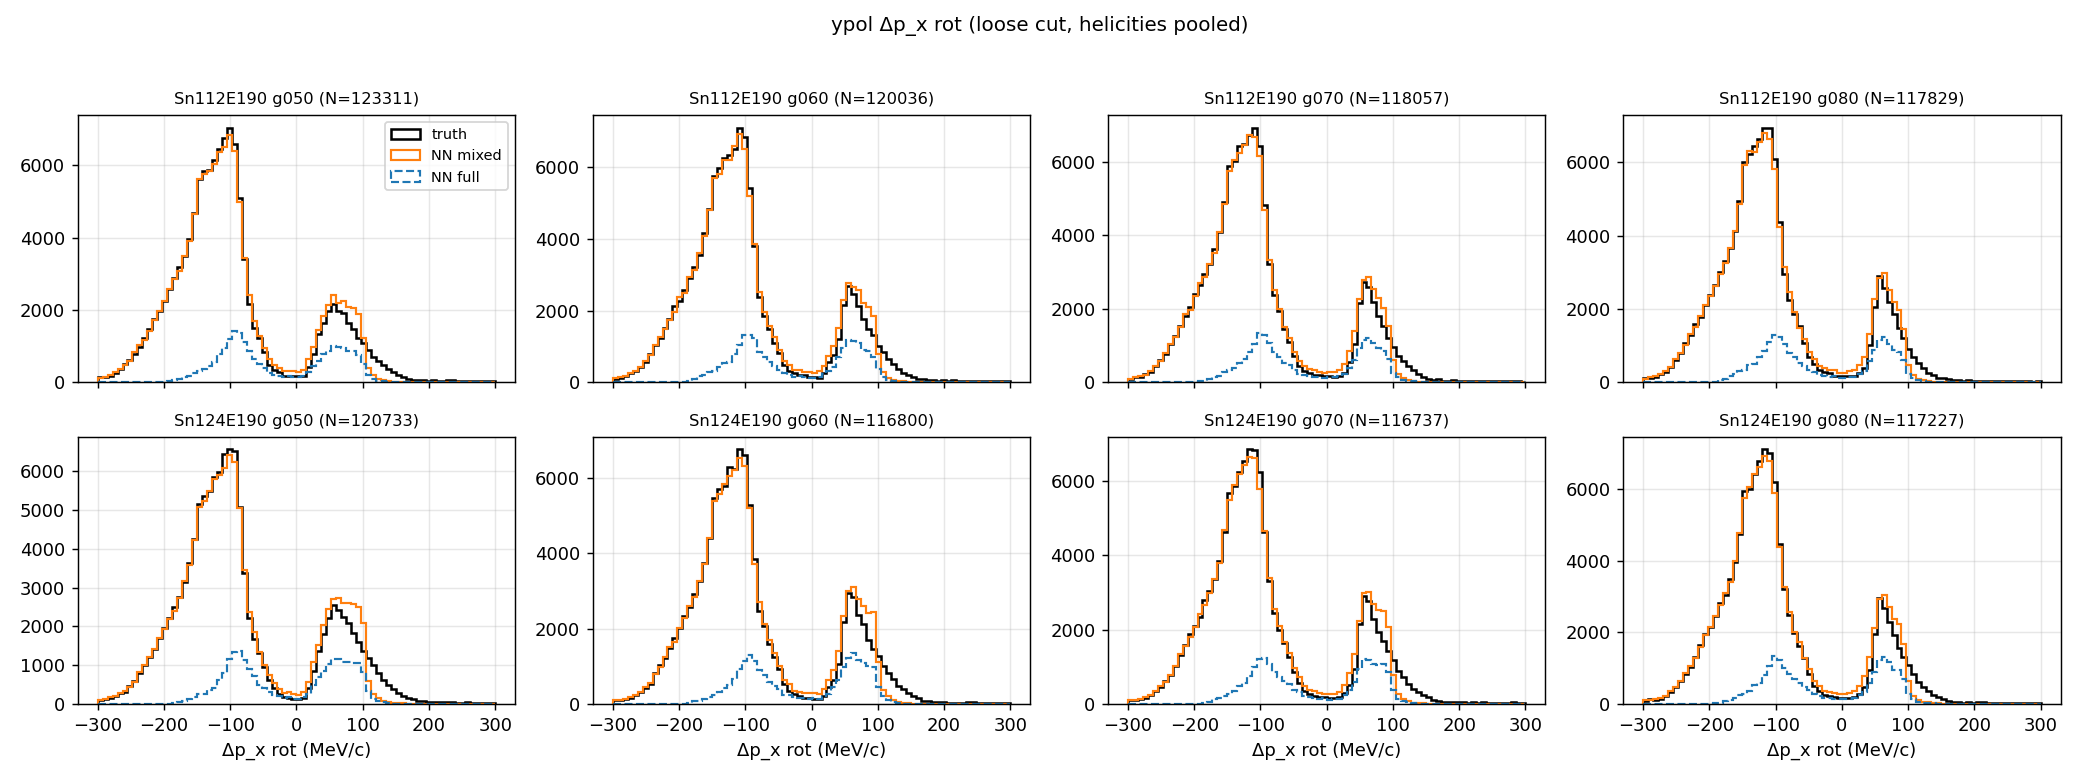
\includegraphics[width=0.85\textwidth]{figures/nn_breakup_phys/px_diff_hist_ypol_loose.png}
\caption{ypol $\Delta p_x^\text{rot}$ 分布 (loose cut). 黑实 = A truth, 橙实 = B NN mixed, 蓝虚 = C NN full. 行 = 2 target, 列 = 4 gamma.}
\end{figure}
\begin{figure}[H]
\centering
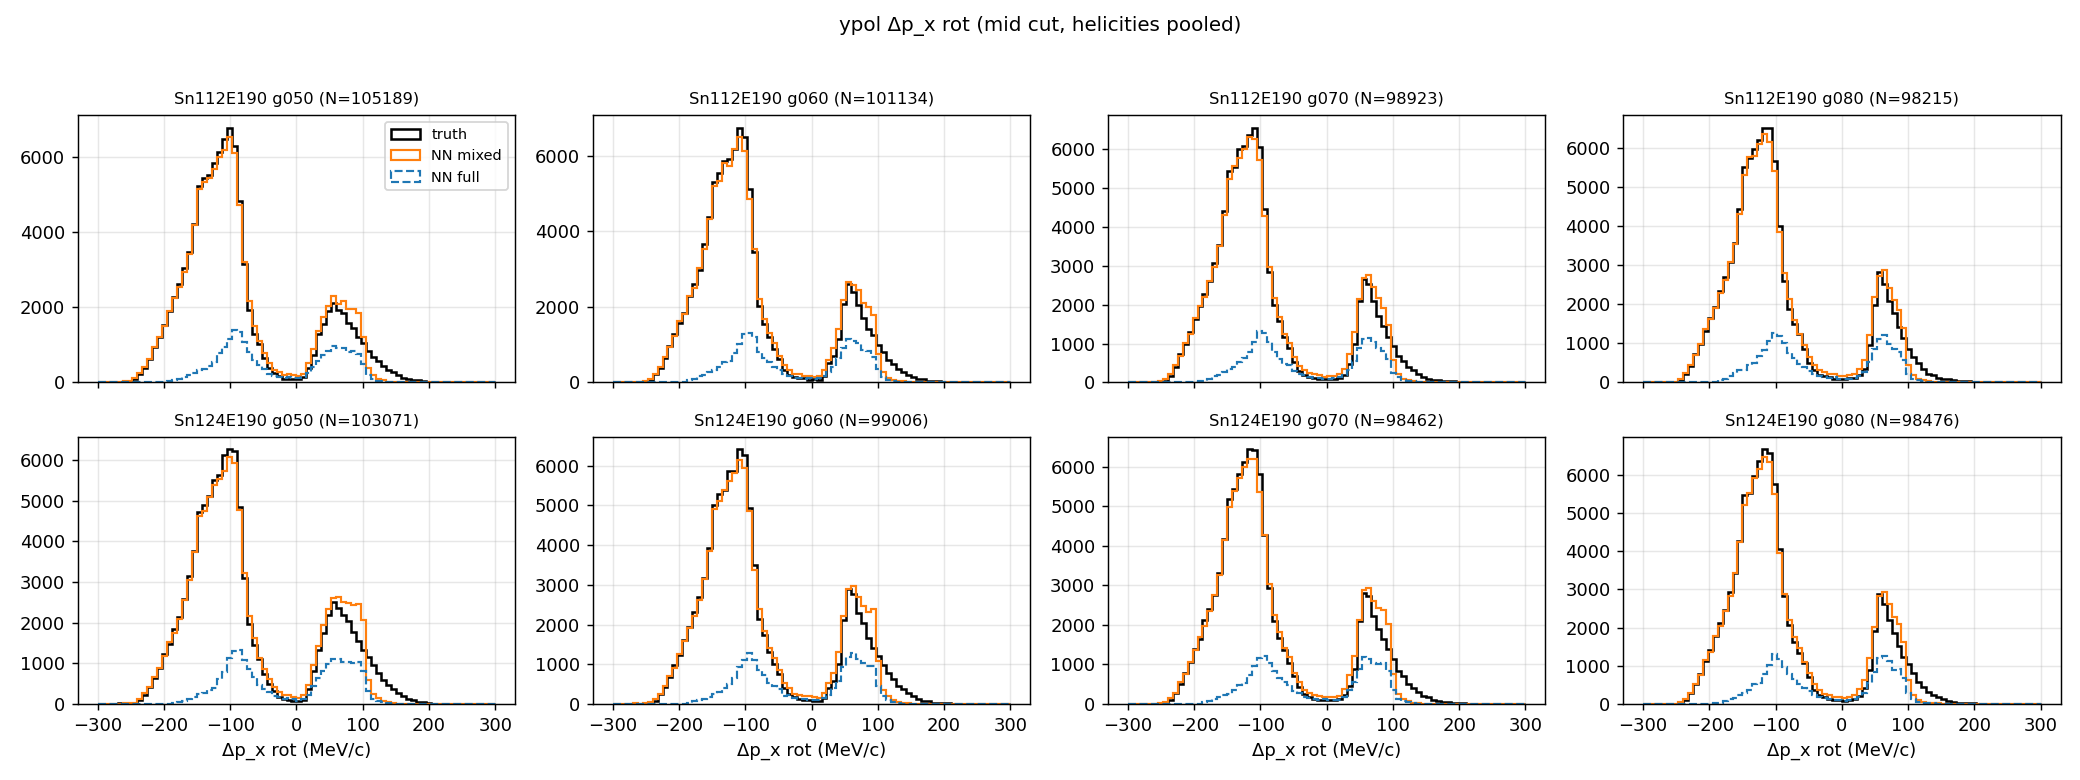
\includegraphics[width=0.85\textwidth]{figures/nn_breakup_phys/px_diff_hist_ypol_mid.png}
\caption{ypol $\Delta p_x^\text{rot}$ 分布 (mid cut).}
\end{figure}
\begin{figure}[H]
\centering
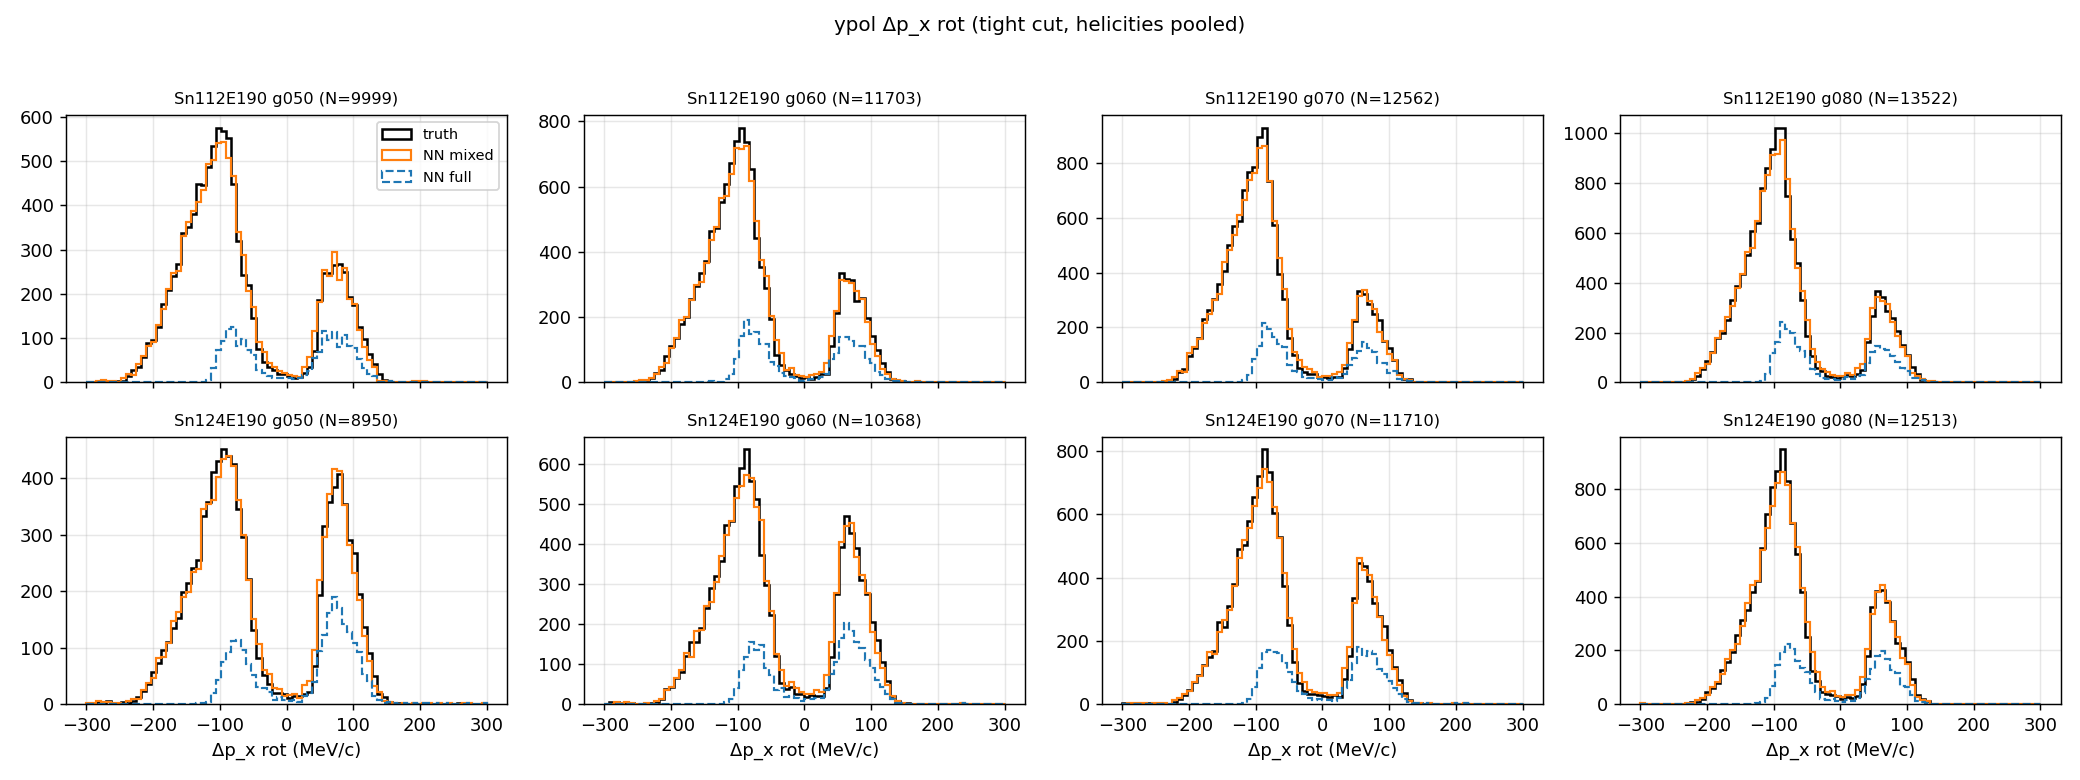
\includegraphics[width=0.85\textwidth]{figures/nn_breakup_phys/px_diff_hist_ypol_tight.png}
\caption{ypol $\Delta p_x^\text{rot}$ 分布 (tight cut).}
\end{figure}

\subsection{5.4 ypol per-particle 残差 (上下游诊断)}

\begin{figure}[H]
\centering
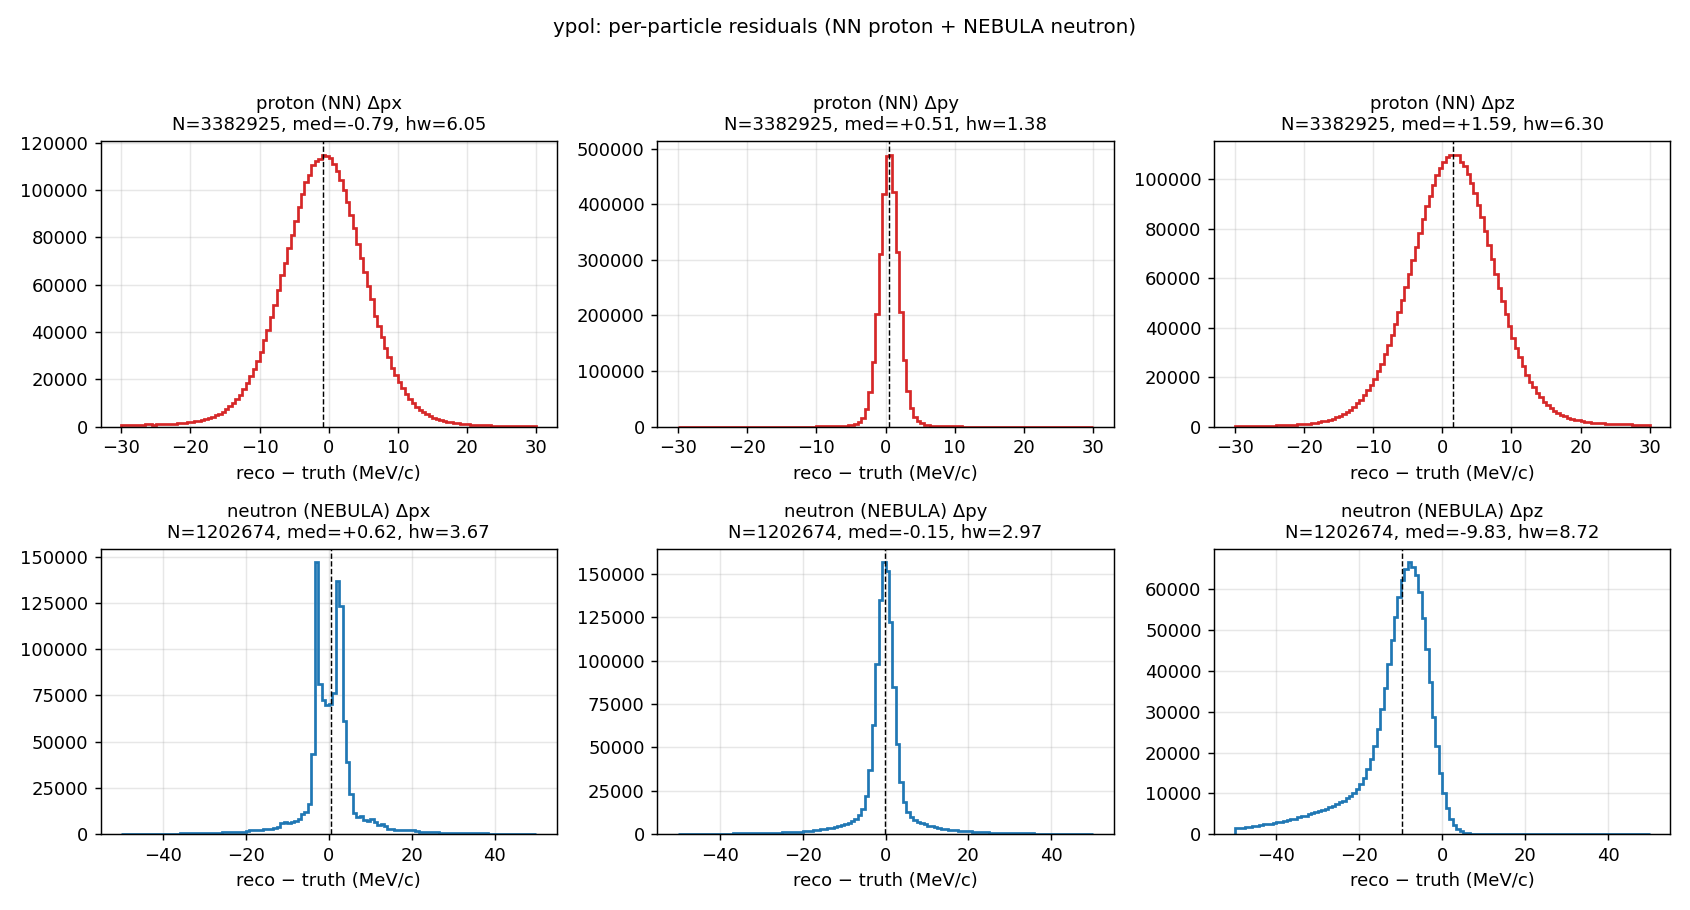
\includegraphics[width=\textwidth]{figures/nn_breakup_phys/residuals_per_particle_ypol.png}
\caption{ypol per-particle 残差. 上行 NN proton (3.38M 事件), 下行 NEBULA neutron (1.20M NEBULA-hit 事件). 黑虚线 = median.}
\end{figure}

\textbf{NN proton}: $\Delta p_x$ med $-0.79$ hw $6.05$, $\Delta p_y$ med $+0.51$ hw $1.38$, $\Delta p_z$ med $+1.59$ hw $6.30$ MeV/$c$. 与 elastic 报告 (\texttt{nn\_vs\_rk\_ypol\_allair\_20260503\_zh.tex} §3.1) 几乎完全一致, 证明 NN 在 breakup 域内的性能与 elastic 域接近.

\textbf{NEBULA neutron}: $\Delta p_z$ med $-9.83$ hw $8.72$ MeV/$c$ — 与 elastic 报告 §1.1 同样的 $\beta$ 法非线性偏置. $\Delta p_x$ 出现明显的双峰 (中央 dip), 这是 NEBULA bar 横向位置由两端时间差离散反推的结构性 artefact, 在 breakup 比 elastic 更明显 (NEBULA 击中率更高, 统计放大了离散步进).

\subsection{5.5 ypol reco vs truth 二维对照}
\begin{figure}[H]
\centering
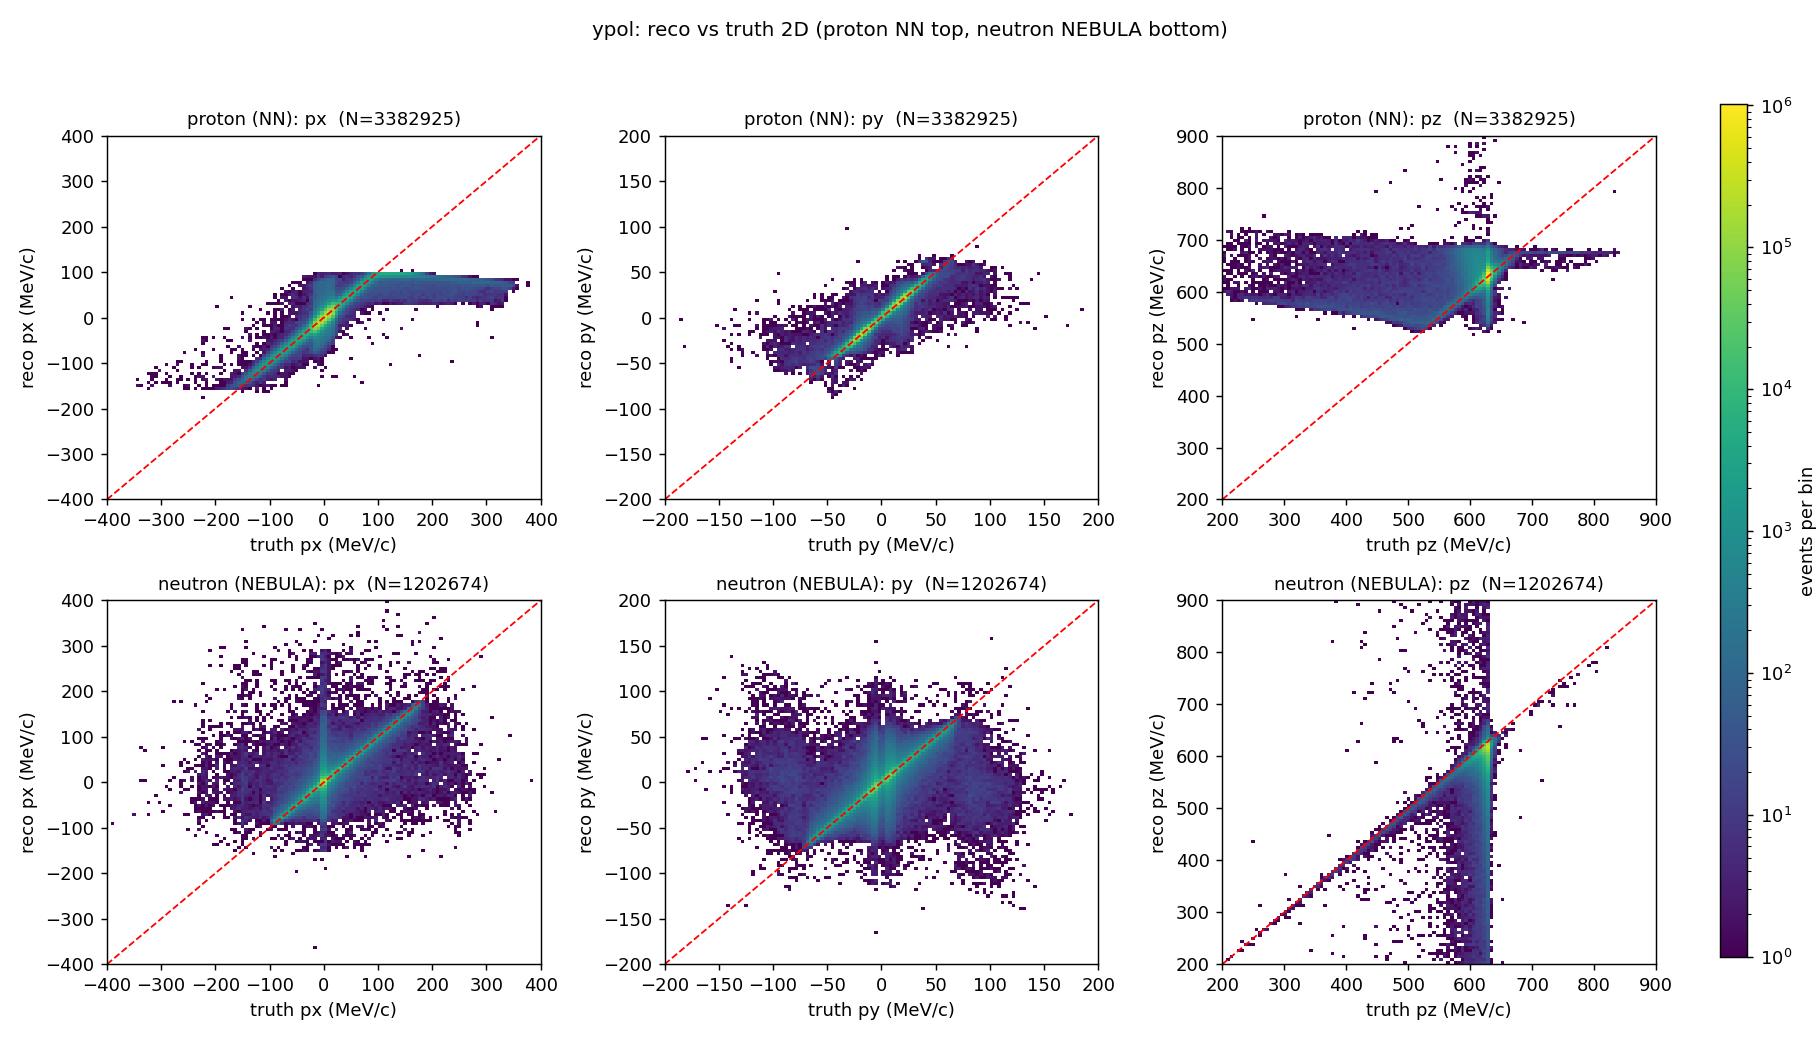
\includegraphics[width=\textwidth]{figures/nn_breakup_phys/reco_vs_truth_2d_ypol.png}
\caption{ypol reco vs truth 2D 直方图. 上行 NN proton (3.38M 事件), 下行 NEBULA neutron (1.20M NEBULA-hit 事件). 红虚线 $y=x$. 6 panel 共享 \texttt{LogNorm} 颜色映射, 右侧 colorbar 标出每 bin 事件数. proton 在 $p_x, p_y$ 方向覆盖 $\pm 400 / \pm 200$ MeV/$c$ 的 breakup 动量范围 (训练域只到 $|p_T|\le 100$, 域外区域可见对角线偏离); $p_z$ 主要堆积在 $\sim 627$ 附近. neutron $p_x$ 上能看到 NEBULA bar 离散步进的横向带状结构.}
\end{figure}

\section{6. zpol 章节}

\subsection{6.1 通过率 (znp+zpn 已合并)}

\begin{table}[H]
\centering\footnotesize
\caption{zpol per-(target, gamma) 通过率.}
\begin{tabular}{llrrrrr}
\toprule
target & gamma & N\_raw & N\_loose & N\_mid & N\_tight & N\_NEBULA(in tight) \\
\midrule
Sn112E190 & g050 &  6\,492 &  6\,393 &  4\,275 & 1\,066 & 236 \\
Sn112E190 & g060 & 10\,255 & 10\,167 &  7\,076 & 1\,751 & 374 \\
Sn112E190 & g070 & 17\,030 & 16\,944 &  9\,543 & 2\,428 & 545 \\
Sn112E190 & g080 & 30\,002 & 29\,914 & 12\,110 & 2\,984 & 789 \\
Sn124E190 & g050 &  4\,885 &  4\,820 &  3\,590 & 1\,101 & 342 \\
Sn124E190 & g060 &  5\,351 &  5\,262 &  3\,774 & 1\,114 & 305 \\
Sn124E190 & g070 &  9\,402 &  9\,321 &  5\,627 & 1\,581 & 438 \\
Sn124E190 & g080 & 18\,245 & 18\,162 &  8\,890 & 2\,395 & 708 \\
\bottomrule
\end{tabular}
\end{table}

\textbf{读法}: zpol 的 loose cut 几乎全过 (98--99\%), 因为 zpol loose 主要由 $p_z$ 重质心条件决定, 几乎无筛选. mid cut 才把 transverse 信息引入, 通过率降到 50--75\%. tight 通过率 13--25\%. NEBULA 在 tight 子集上击中率 22--32\%.

\subsection{6.2 R 表 (zpol)}

\begin{table}[H]
\centering\scriptsize
\caption{zpol $R_x^\text{rot}$ (反应平面 frame, znp+zpn pooled).}
\begin{tabular}{ll|ccc|ccc|ccc}
\toprule
& & \multicolumn{3}{c|}{\textbf{loose}} & \multicolumn{3}{c|}{\textbf{mid}} & \multicolumn{3}{c}{\textbf{tight}} \\
target & gamma & A truth & B mixed & C full & A truth & B mixed & C full & A truth & B mixed & C full \\
\midrule
Sn112 & g050 & 0.147 & 0.141 & 0.220 & 0.142 & 0.152 & 0.269 & 0.213 & 0.218 & 0.466 \\
Sn112 & g060 & 0.091 & 0.086 & 0.136 & 0.097 & 0.103 & 0.175 & 0.154 & 0.160 & 0.345 \\
Sn112 & g070 & 0.165 & 0.166 & 0.233 & 0.076 & 0.089 & 0.149 & 0.115 & 0.116 & 0.208 \\
Sn112 & g080 & 0.290 & 0.296 & 0.363 & 0.050 & 0.065 & 0.111 & 0.079 & 0.095 & 0.199 \\
Sn124 & g050 & 0.949 & 0.841 & 1.233 & 0.941 & 0.935 & 1.536 & 1.363 & 1.343 & 3.622 \\
Sn124 & g060 & 0.531 & 0.462 & 0.631 & 0.606 & 0.594 & 0.867 & 0.885 & 0.829 & 1.563 \\
Sn124 & g070 & 0.351 & 0.335 & 0.435 & 0.355 & 0.371 & 0.532 & 0.507 & 0.532 & 0.982 \\
Sn124 & g080 & 0.312 & 0.312 & 0.374 & 0.225 & 0.249 & 0.341 & 0.298 & 0.325 & 0.532 \\
\bottomrule
\end{tabular}
\end{table}

完整 CI 见 \texttt{summary/zpol/r\_table.csv}.

\textbf{物理结论}:
\begin{itemize}[nosep]
    \item \textbf{Sn124 信号最显著}, tight cut 下 R 从 1.36 (g050) 跌到 0.30 (g080), 横跨 4 倍, 比 ypol Sn124 信号更强.
    \item \textbf{Sn112 趋势非单调}: loose 在 g060 处反跳, mid/tight 在 g070-g080 单调下降但绝对值很小. 统计有限 (per cell 几千事件), 趋势可能受统计涨落影响; bootstrap CI 见原始 csv.
    \item \textbf{B mixed 与 A truth} 在 zpol Sn124 loose g050/g060 处偏差较大 (0.95 vs 0.84, $\sim$11\%); 其他位置 $<5\%$. 这一偏差可能是 NN proton 与 NEBULA neutron-fallback 的统计互不独立带来的偏置 (zpol 样本小, 该效应放大), 也值得在 RK 比较中验证.
    \item \textbf{C full reco}: 仅在 NEBULA-hit 子集上, 受同样的接收度偏置.
\end{itemize}

\subsection{6.3 zpol R 与 $\Delta p_x^\text{rot}$ 图}

\begin{figure}[H]
\centering
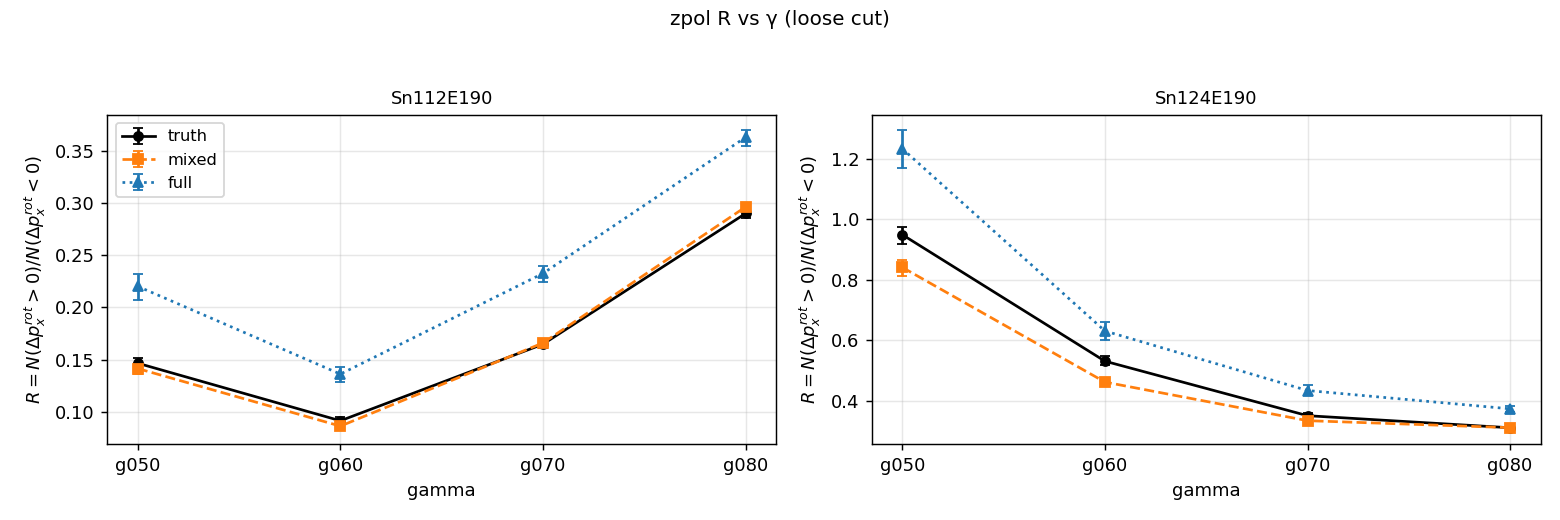
\includegraphics[width=0.95\textwidth]{figures/nn_breakup_phys/r_vs_gamma_zpol_loose.png}
\caption{zpol $R_x^\text{rot}$ vs gamma (loose cut).}
\end{figure}
\begin{figure}[H]
\centering
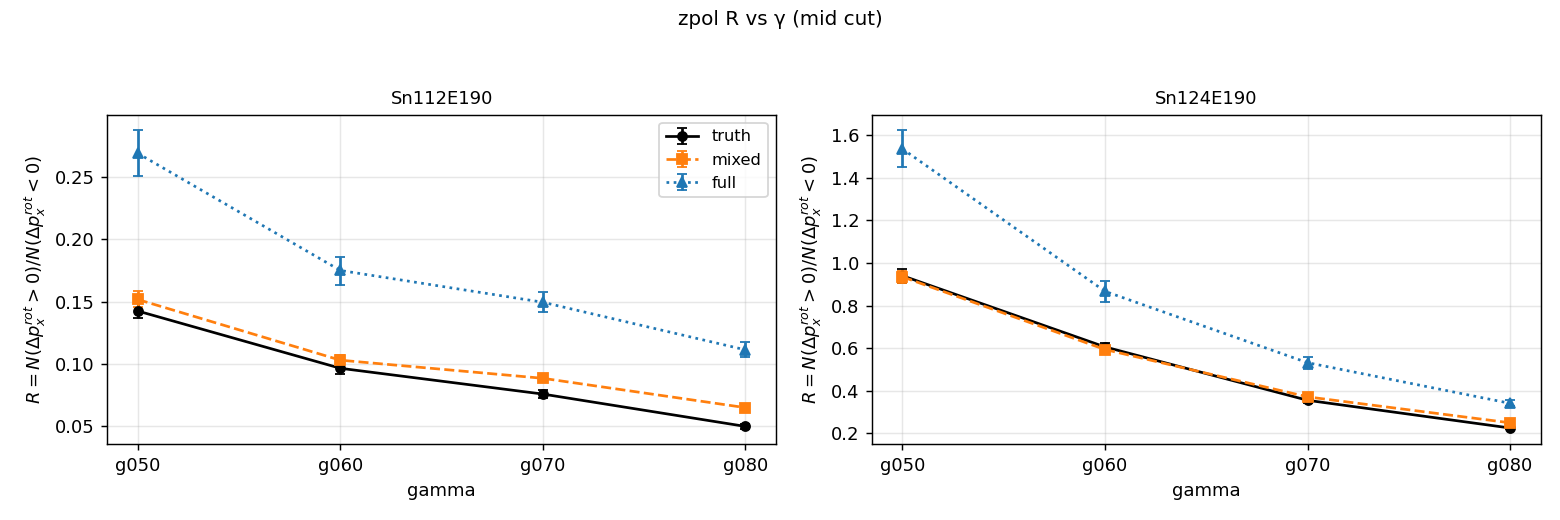
\includegraphics[width=0.95\textwidth]{figures/nn_breakup_phys/r_vs_gamma_zpol_mid.png}
\caption{zpol $R_x^\text{rot}$ vs gamma (mid cut).}
\end{figure}
\begin{figure}[H]
\centering
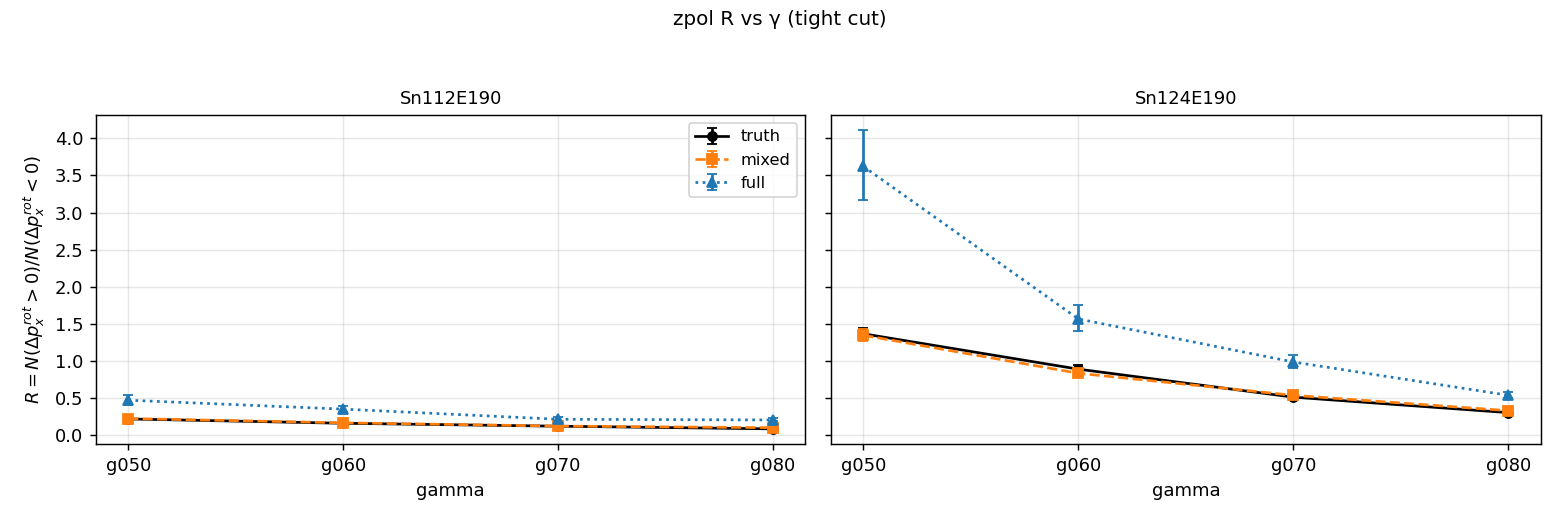
\includegraphics[width=0.95\textwidth]{figures/nn_breakup_phys/r_vs_gamma_zpol_tight.png}
\caption{zpol $R_x^\text{rot}$ vs gamma (tight cut).}
\end{figure}

\begin{figure}[H]
\centering
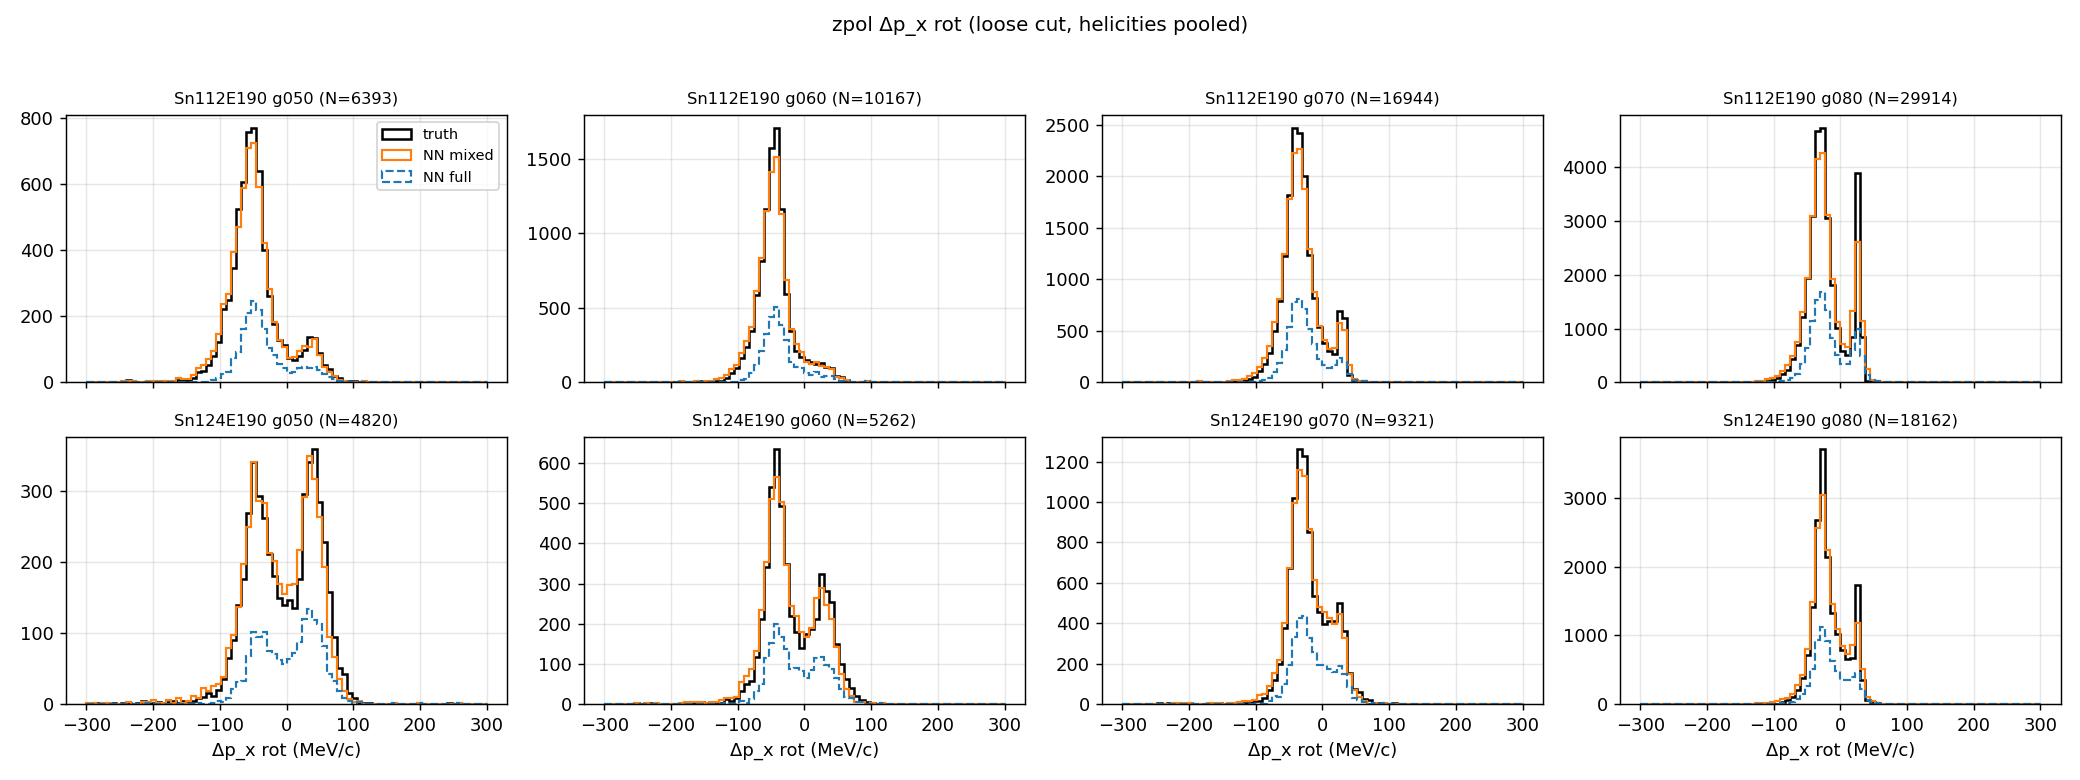
\includegraphics[width=0.85\textwidth]{figures/nn_breakup_phys/px_diff_hist_zpol_loose.png}
\caption{zpol $\Delta p_x^\text{rot}$ 分布 (loose cut).}
\end{figure}
\begin{figure}[H]
\centering
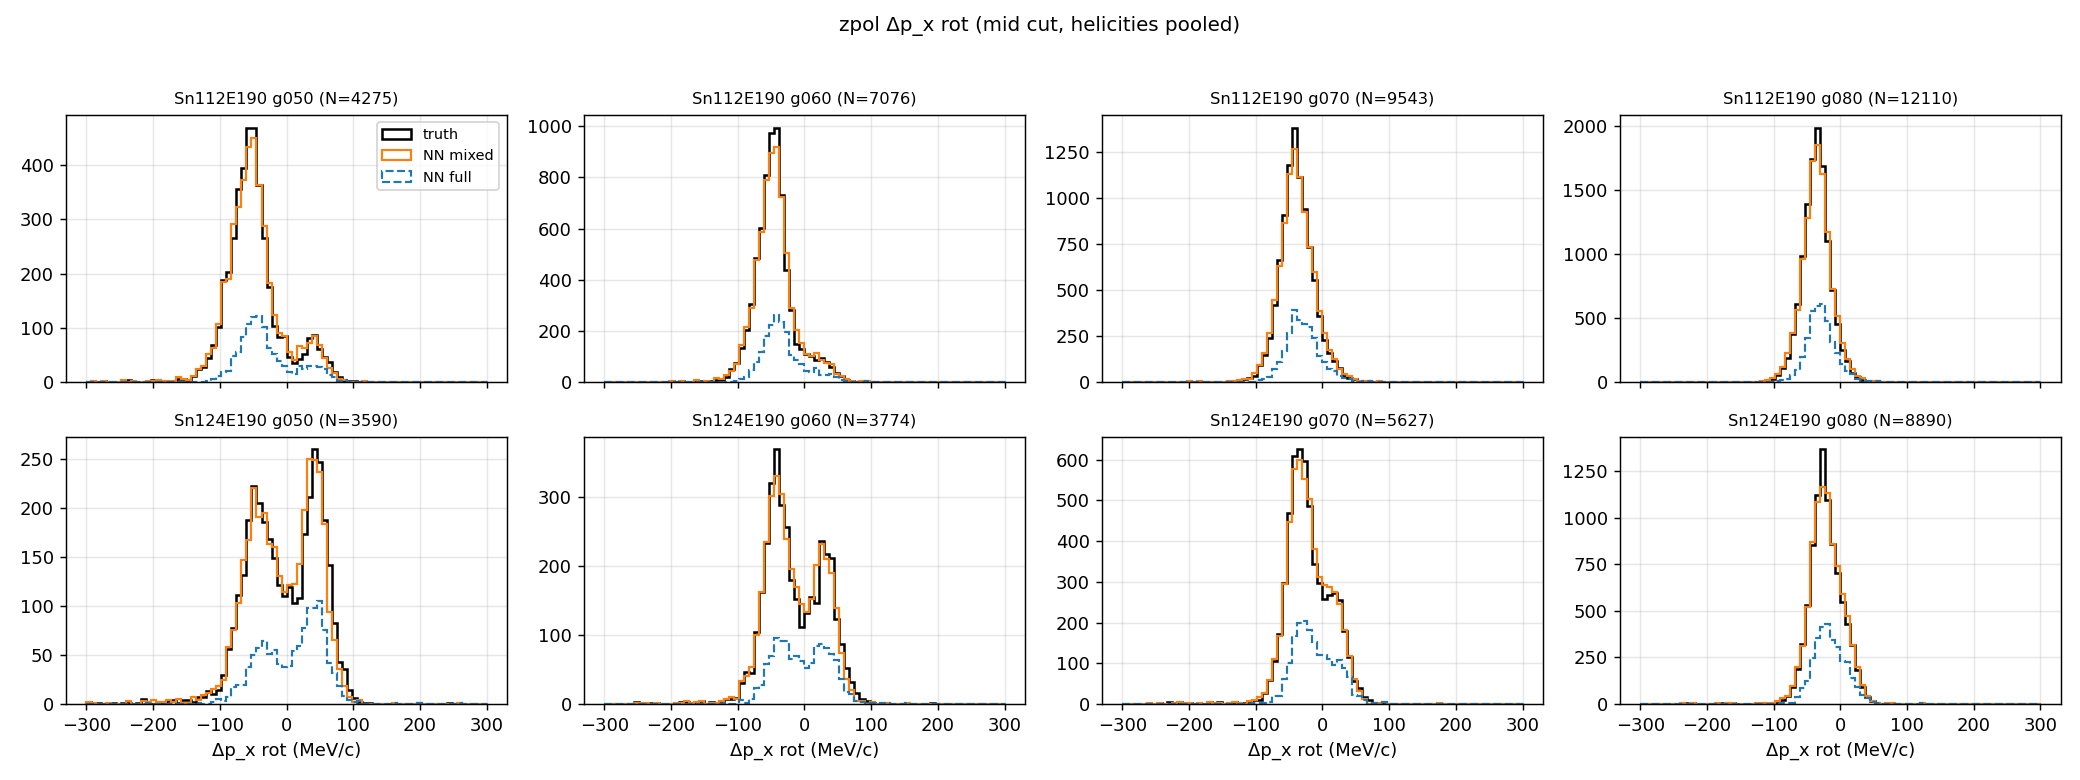
\includegraphics[width=0.85\textwidth]{figures/nn_breakup_phys/px_diff_hist_zpol_mid.png}
\caption{zpol $\Delta p_x^\text{rot}$ 分布 (mid cut).}
\end{figure}
\begin{figure}[H]
\centering
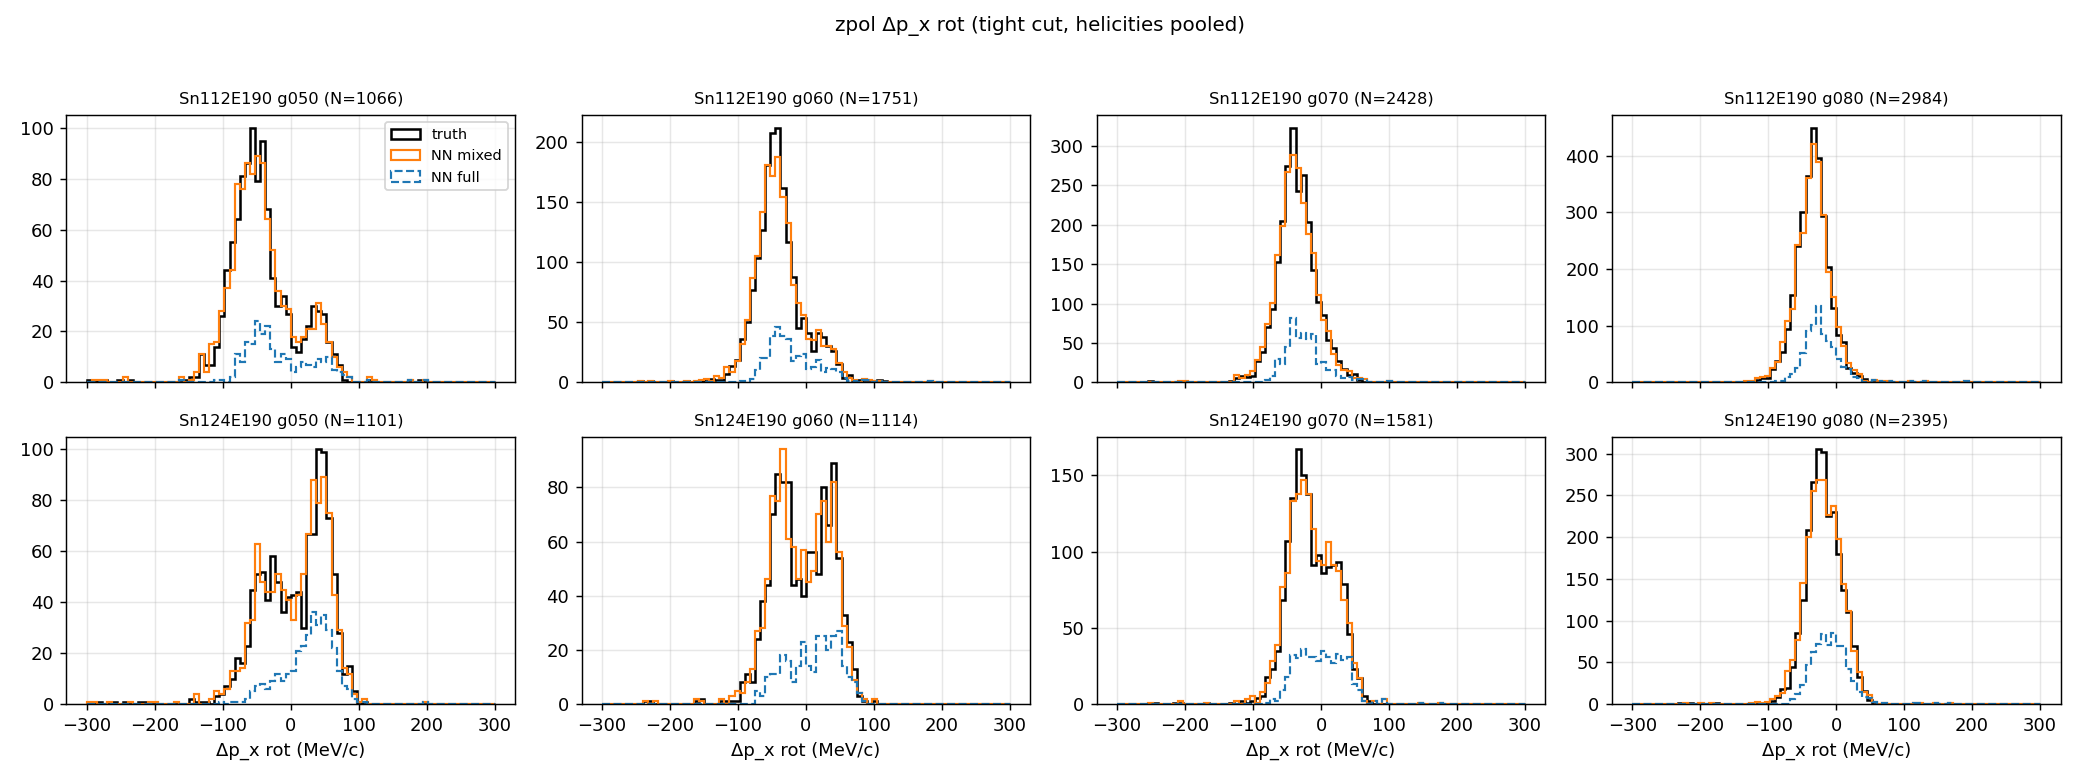
\includegraphics[width=0.85\textwidth]{figures/nn_breakup_phys/px_diff_hist_zpol_tight.png}
\caption{zpol $\Delta p_x^\text{rot}$ 分布 (tight cut).}
\end{figure}

\subsection{6.4 zpol per-particle 残差}

\begin{figure}[H]
\centering
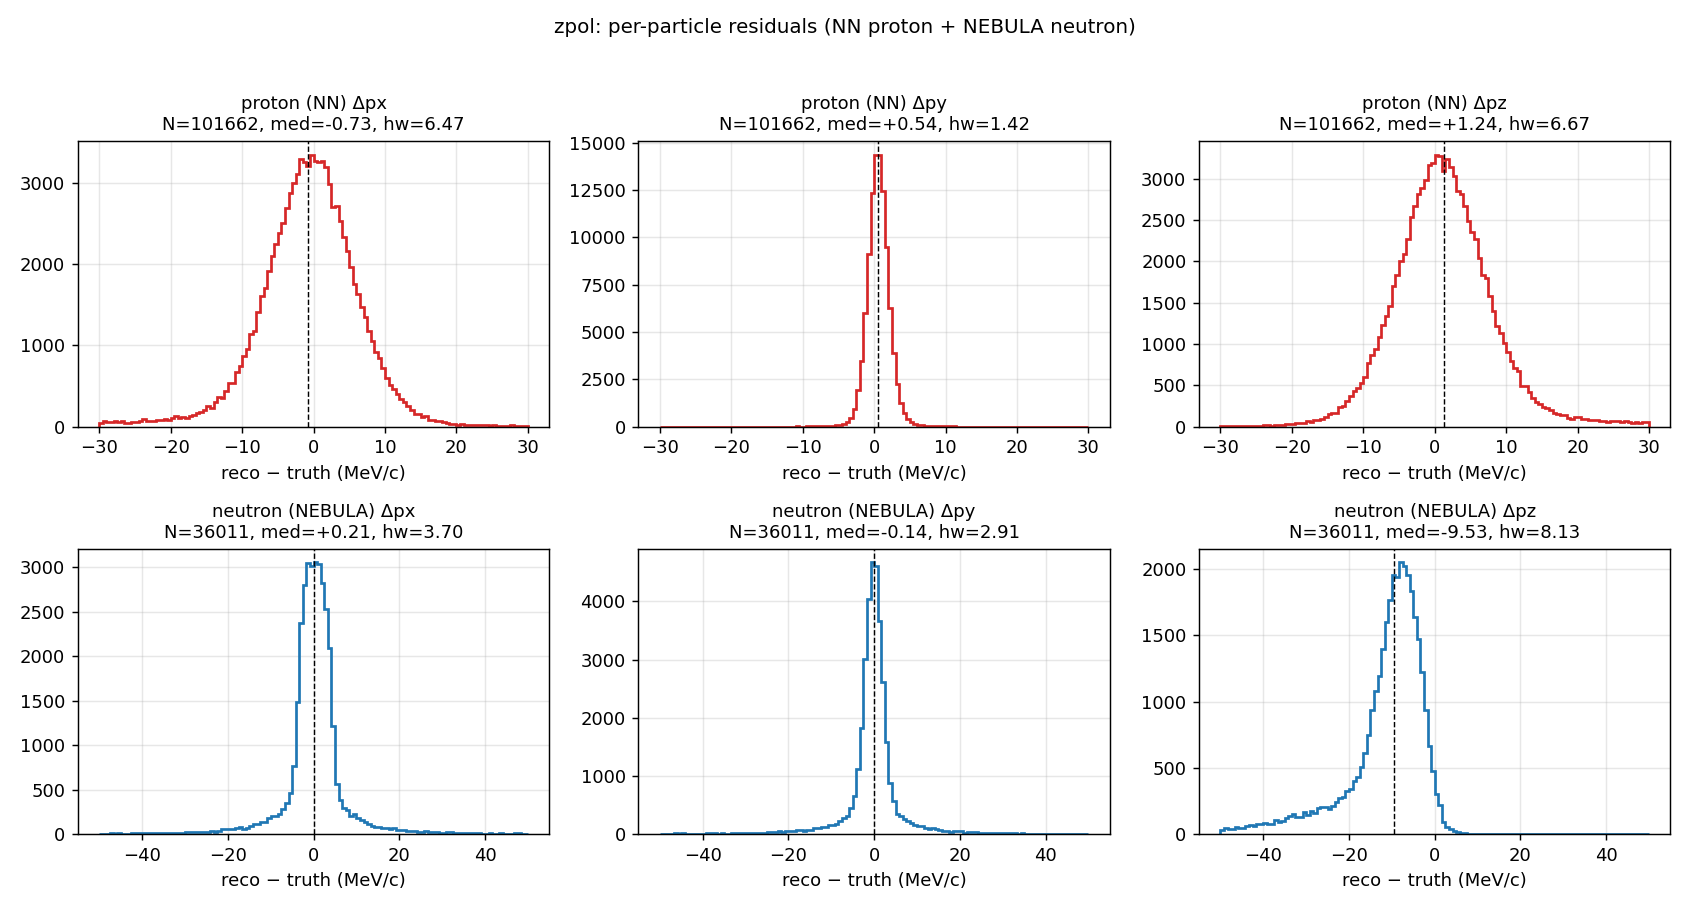
\includegraphics[width=\textwidth]{figures/nn_breakup_phys/residuals_per_particle_zpol.png}
\caption{zpol per-particle 残差. 上行 NN proton, 下行 NEBULA neutron.}
\end{figure}

注意 zpol 训练域覆盖率 91.3\% (vs ypol 97.4\%), 残差略宽于 ypol 但量级相同; 不构成 R 比值的显著扰动.

\subsection{6.5 zpol reco vs truth 二维对照}
\begin{figure}[H]
\centering
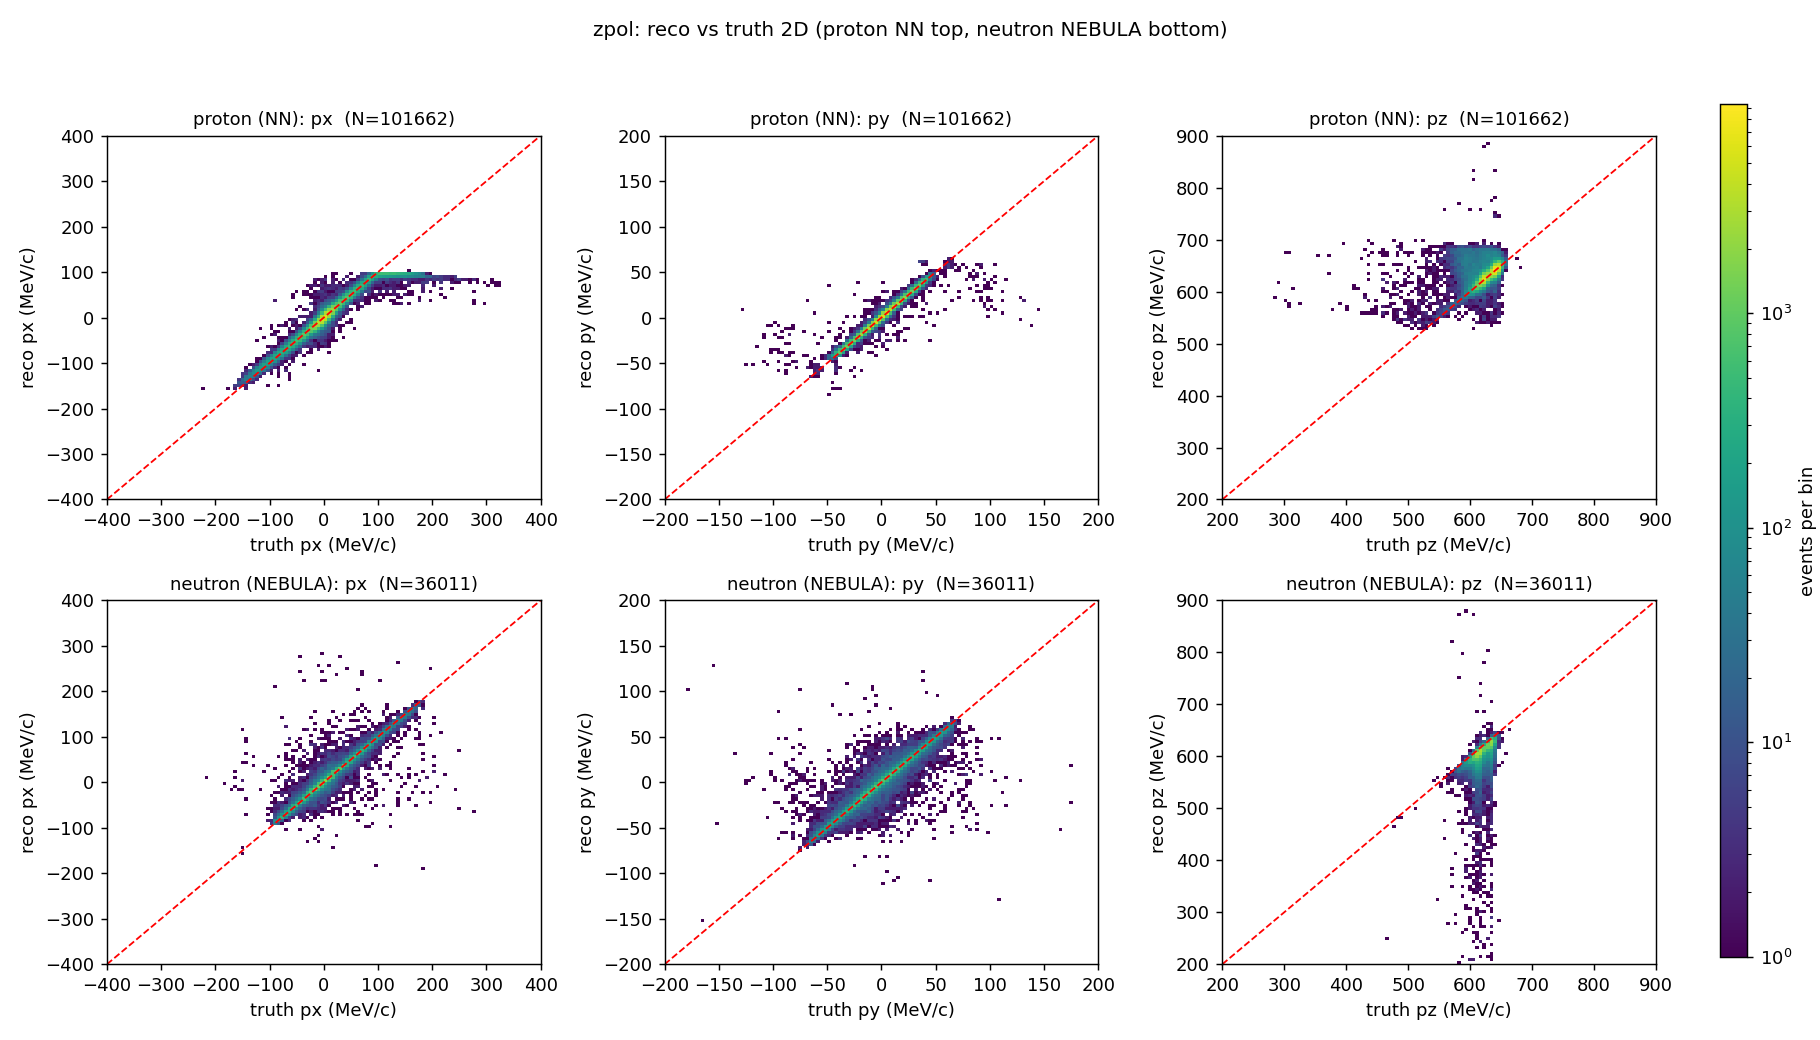
\includegraphics[width=\textwidth]{figures/nn_breakup_phys/reco_vs_truth_2d_zpol.png}
\caption{zpol reco vs truth 2D 直方图. 上行 NN proton, 下行 NEBULA neutron. 红虚线 $y=x$. 6 panel 共享 \texttt{LogNorm} 颜色映射, 右侧 colorbar 标出每 bin 事件数. proton 在域外 ($|p_T| > 100$ MeV/$c$) 处可见对角线弯折; neutron 与 ypol 同样存在 NEBULA 离散步进结构.}
\end{figure}

\section{7. 结论 \& 下一步}

\begin{enumerate}[nosep]
    \item 主 NN 模型在 breakup g4output 上 forward 推理稳定, 100\% 给出 proton 输出.
    \item ypol Sn124 R 信号清晰, 三档 cut 下都呈 gamma 单调下降; zpol Sn124 信号更强, R 跨度更大.
    \item NN B mixed 与 A truth 在 ypol 上一致到 $<3\%$, zpol 上 $<11\%$; 后者偏差归因于小统计 + neutron-fallback 互依赖, 待 RK 比较验证.
    \item NN proton 残差 $\sigma$ 在 breakup 上与 elastic 一致, 训练域覆盖 ypol 97\% / zpol 91\%, 不显著外推.
\end{enumerate}

\textbf{后续报告}:
\begin{itemize}[nosep]
    \item \textbf{下一份}: 同样 spana03 g4output 上, 用 RK 重建 (在 spana03 上跑后) 出独立报告 \texttt{rk\_breakup\_phys\_<date>\_zh.tex}.
    \item \textbf{下下份}: \texttt{nn\_vs\_rk\_breakup\_phys\_<date>\_zh.tex} 头对头比较, 重点观察 (a) NN 是否在大 $p_T$ 外推区显著差于 RK, (b) 二者 R 偏差是否来自共同的 NEBULA 系统效应.
\end{itemize}

\section*{Artifacts}
\begin{itemize}[nosep]
    \item rsync 脚本: \texttt{scripts/analysis/nn\_breakup\_phys/00\_rsync\_from\_spana03.sh}
    \item NN reco driver: \texttt{scripts/analysis/nn\_breakup\_phys/01\_run\_nn\_reco.sh}
    \item 抽取宏: \texttt{scripts/analysis/nn\_breakup\_phys/02\_extract\_observables.C}
    \item 抽取驱动: \texttt{scripts/analysis/nn\_breakup\_phys/run\_extract\_all.sh}
    \item R/$\Delta p_x$ 分析: \texttt{scripts/analysis/nn\_breakup\_phys/03\_analyze\_r\_breakup.py}
    \item 绘图: \texttt{scripts/analysis/nn\_breakup\_phys/04\_make\_figures.py}
    \item NN reco 输出 ROOT: \texttt{data/reconstruction/breakup\_nn\_20260503/\{y\_pol,z\_pol\}/}
    \item 中间 CSV: \texttt{build/test\_output/nn\_breakup\_phys\_20260503/csv/\{ypol,zpol\}/}
    \item R 表 / 通过率 / 联合 df: \texttt{build/test\_output/nn\_breakup\_phys\_20260503/summary/\{ypol,zpol\}/}
\end{itemize}

\end{document}
